\ifdefined\ismainfile
\else
    \documentclass[11pt]{article}

    \makeatletter
\@ifclassloaded{revtex4-2}{}{\usepackage[margin=1in]{geometry}}
\makeatother
\usepackage{amsmath,amsthm,amsfonts,amssymb,mathrsfs}
\usepackage{graphicx}
\usepackage{cancel}
\usepackage{bm}
\usepackage{tikz}
\usepackage{csquotes}
\usepackage{tikz-3dplot}
\usepackage{physics}
\usepackage{dsfont}
\usepackage{float}
\usepackage{xcolor}
\usepackage{mathtools}
\usepackage{tcolorbox}
\makeatletter
\@ifclassloaded{revtex4-2}{\let\affil\affiliation
}{\usepackage{authblk}}
\makeatother

\tcbuselibrary{breakable}
\usepackage{keytheorems}
\newkeytheorem{definition}[parent=section, tcolorbox-no-titlebar={breakable, colback=blue!10}]
\newkeytheorem{example,lemma,conjecture,claim,theorem,proposition,corollary,fact,assumption,construction}[sibling=definition, tcolorbox-no-titlebar={breakable, colback=blue!10}]
\theoremstyle{definition}
\newtheorem{protocol}{Protocol}[section]

\newkeytheorem{remark}[parent=section, tcolorbox-no-titlebar={breakable}]
\allowdisplaybreaks[4]
\interdisplaylinepenalty=0
\makeatletter
\renewcommand{\log}{\mathop{\operator@font log}\nolimits}
\makeatother
\IfFileExists{bbm.sty}{\usepackage{bbm}}{\providecommand{\mathbbm}{\mathds}}
\usepackage{stmaryrd}
\usepackage{braket}
\makeatletter
\@ifpackageloaded{natbib}{}{\usepackage[numbers,sort&compress]{natbib}}
\makeatother
\usepackage{hyperref}
\usepackage[ruled,noline,longend]{algorithm2e}
\SetAlgoNoLine
\AtBeginDocument{\SetAlgoNoLine}
\SetAlgoLongEnd
\RestyleAlgo{boxruled}
\LinesNumbered
\definecolor{algcommentgray}{gray}{0.35}
\newcommand{\AlgCommentFont}[1]{\textcolor{algcommentgray}{#1}}
\SetCommentSty{AlgCommentFont}
\SetKwComment{tcp}{{\color{algcommentgray}$\blacktriangleright$}\ }{}
\usepackage{tcolorbox}
\tcbuselibrary{breakable}
\renewcommand{\topfraction}{0.9}
\renewcommand{\bottomfraction}{0.8}
\renewcommand{\textfraction}{0.07}
\renewcommand{\floatpagefraction}{0.85}
\setcounter{topnumber}{3}
\setcounter{totalnumber}{5}
\newenvironment{longalgorithm}[2][]{\begin{tcolorbox}[breakable, sharp corners, boxsep=0pt,
      boxrule=\algoheightrule, colframe=black, colback=white,
      left=18pt, right=4pt, top=5pt, bottom=5pt, #1]\refstepcounter{algocf}\noindent\hspace*{-14pt}{\textbf{\algorithmcfname~\thealgocf:} #2}\par
  \addcontentsline{loa}{algocf}{\protect\numberline{\thealgocf}#2}\par\nobreak\vspace{2pt}\nointerlineskip
  \moveleft18pt\vbox{\hrule width \dimexpr\linewidth+22pt\relax height \algoheightrule}\vspace{3pt}\setcounter{AlgoLine}{0}\RestyleAlgo{plain}}{\end{tcolorbox}}
\DontPrintSemicolon
\SetKwInput{KwIn}{Require}
\SetKwInput{KwOut}{Ensure}
\SetKwFor{For}{for}{do}{end for}
\SetKwFor{ForEach}{for each}{do}{end for}
\SetKwFor{While}{while}{do}{end while}
\makeatletter
\newenvironment{breakablealgorithm}{\par\addvspace{\intextsep}\hrule height .8pt\kern2pt
  \renewcommand{\caption}[2][]{\refstepcounter{algocf}\noindent\textbf{\algorithmcfname~\thealgocf:} ##2\par
    \kern2pt\hrule\kern2pt
    \ifx\relax##1\relax
      \addcontentsline{loa}{algocf}{\protect\numberline{\thealgocf}##2}\else
      \addcontentsline{loa}{algocf}{\protect\numberline{\thealgocf}##1}\fi
  }}{\par\kern2pt\hrule\addvspace{\intextsep}}
\makeatother
\usepackage{old-arrows}
\usepackage{color}
\usepackage{array, tabularx}
\usepackage{longtable}
\makeatletter
\@ifclassloaded{revtex4-2}{\appdef\@mkpream@relax{\let\@endpbox\relax}}{}
\makeatother
\usepackage{booktabs}
\newcolumntype{L}[1]{>{\raggedright\arraybackslash}p{#1}}
\newcolumntype{C}[1]{>{\centering\arraybackslash}p{#1}}
\newcolumntype{R}[1]{>{\raggedleft\arraybackslash}p{#1}}
\newcommand{\Circo}[0]{\mathfrak{C}}
\newcommand{\restrict}[2]{#1 \vert_{#2}}
\newcommand{\physq}[0]{\mathcal{M}}


\newcommand{\Xp}[0]{\mathcal{X}}
\newcommand{\Zp}[0]{\mathcal{Z}}

\newcommand{\nS}[1]{\mathbb{N}_{#1}}
\newcommand{\aS}[1]{\mathbb{C}_{#1}}

\newcommand{\nD}[1]{D^N_{#1}}
\newcommand{\aD}[1]{D^C_{#1}}

\newcommand{\control}[3]{C_{#1} {#2}_{#3}}
\usetikzlibrary{3d, shapes, arrows.meta, decorations.pathreplacing, decorations.markings, cd, shapes.geometric, calc}
\IfFileExists{tikzlibrarycalligraphy.code.tex}{\usetikzlibrary{calligraphy}}{}
\pgfkeysifdefined{/pgf/decoration/calligraphic brace/.@cmd}{}{\pgfkeys{/pgf/decoration/calligraphic brace/.style={brace}}}
\tikzstyle{midarrow} = [decoration={markings, mark= at position 0.6 with {\arrow{Stealth}}}, postaction={decorate}]
\renewcommand{\comment}[1]{{\color{red} #1}}

\newcommand{\YR}[1]{{\color{Teal} [Collin: #1]}}

\newcommand{\kc}[1]{{\color{cyan} [Katie: #1]}}

\newcommand{\bb}[1]{{\color{purple}[BB: #1]}}




\newcommand{\vva}[1]{{\color{magenta} [VVA: #1]}}









\newcommand{\al}[1]{{\color{DarkGreen} [Ana: #1]}}

\newcommand{\hp}[1]{{\color{brown} [Harry: #1]}}

\newcommand{\NT}[1]{{\color{orange} [NT: #1]}}

\newcommand{\dom}[1]{\textcolor{blue}{[Dom: #1]}}

\newcommand{\todo}[1]{\textcolor{blue}{[TO-DO: #1]}}

\newcommand{\new}[1]{{\color{DarkMagenta}#1}}
\definecolor{FGreen}{RGB}{58,158,92}
\definecolor{lightred}{RGB}{223, 123, 84}
\definecolor{lightbrown}{RGB}{242,216,199}
\definecolor{invisiblegray}{RGB}{238,238,237}
\definecolor{lightgreen}{RGB}{222, 235, 218}
\definecolor{lightcyan}{RGB}{153, 191, 216}
\definecolor{lightcyan2}{RGB}{208, 224, 235}
\definecolor{cyan2}{RGB}{144,201,226}
\definecolor{lightyellow}{RGB}{252, 238, 183}
\definecolor{OrangeRed}{RGB}{223,123,84}
\definecolor{CyanGreen}{RGB}{81,177,184}
\definecolor{rose}{RGB}{226,45,139}
\definecolor{Ycolor}{RGB}{248,236,104}
\definecolor{Hcolor}{RGB}{255,255,0}
\definecolor{Xcolor}{RGB}{246,143,138}
\definecolor{Zcolor}{RGB}{210,254,206}
\definecolor{Lred}{RGB}{244,163,163}
\definecolor{Lgreen}{RGB}{160,211,179}
\definecolor{Lblue}{RGB}{170,183,240}
\definecolor{tickcolor}{RGB}{181,0,250}
\definecolor{DarkBlue}{RGB}{14,38,80}
\definecolor{greenblue}{RGB}{0,255,127}
\definecolor{darkblue}{RGB}{57,85,134}
\definecolor{electrored}{RGB}{244,96,85}
\definecolor{electrored2}{RGB}{245,107,94}
\definecolor{BBXcheck}{RGB}{210,234,206}
\definecolor{BBZcheck}{RGB}{204,204,250}
\definecolor{softred}{RGB}{245,206,206}
\definecolor{fuchsiapurple}{RGB}{180, 0, 255}
\definecolor{Teal}{RGB}{62,138,141}
\definecolor{gold}{RGB}{233,168,58}
\definecolor{Crimson}{RGB}{220,20,60}
\definecolor{RedOrange}{RGB}{255,69,0}
\definecolor{DarkMagenta}{RGB}{139,0,139}
\definecolor{DarkGreen}{RGB}{0,100,0}
\definecolor{MidnightBlue}{RGB}{25,25,112}



\newcommand{\g}{\mathbf{g}}
\newcommand{\h}{\mathbf{h}}
\renewcommand{\k}{\mathbf{k}}
\newcommand{\f}{\mathbf{f}}
\newcommand{\C}{\mathbf{C}}
\newcommand{\Z}{\mathbb{Z}}
\renewcommand{\S}{\mathcal{S}}
\newcommand{\CC}{\mathcal{C}}
\newcommand{\charge}{k}
\newcommand{\totalcharge}{K}
\newcommand{\B}{\mathbb{B}}
\renewcommand{\O}{\mathcal{O}}
\newcommand{\Ocal}{\mathcal{O}}
\renewcommand{\Vec}{\mathcal{V}ec}
\newcommand{\Rep}{\text{Rep}}
\newcommand{\nnb}{\nonumber}
\newcommand{\lt}{\triangleleft}
\newcommand{\rt}{\triangleright}
\newcommand{\Lcal}{\mathcal{L}}
\newcommand{\Acal}{\mathcal{A}}
\newcommand{\Gcal}{\mathcal{G}}
\newcommand{\XX}{\mathcal{X}}
\newcommand{\YY}{\mathcal{Y}}
\newcommand{\ZZ}{\mathcal{Z}}
\newcommand{\Com}[2]{[ #1, #2 ]}
\newcommand{\ComGrp}[2]{[ #1, #2 ]_{\text{grp}}}
\newcommand{\level}{\operatorname{Lv}}
\newcommand{\code}{\mathcal{C}}


\newcommand{\glosym}[0]{\mathsf{L}}
\newcommand{\im}{\operatorname{im}}
\newcommand{\rk}{\operatorname{rk}}
\newcommand{\supp}[1]{\operatorname{Supp}(#1)}
\newcommand{\Ad}{\operatorname{Ad}}
\newcommand{\Irrep}{\operatorname{Irrep}}
\newcommand{\Wt}{\operatorname{Wt}}
\newcommand{\Lin}{\mathfrak{L}}
\newcommand{\interior}{\operatorname{int}}
\newcommand{\T}[0]{\mathsf{U}}
\newcommand{\orbit}[1]{O^{\mathcal{T}}(#1)}
\newcommand{\sym}[0]{\overline{S}}
\newcommand{\av}[0]{\mathbb{A}_v}
\newcommand{\bp}[0]{\mathbb{B}_f}
\newcommand{\onsite}[1]{\mathsf{T}|_{#1}}
\newcommand{\Log}[1]{\overline{#1}}
\newcommand{\id}[0]{\mathbf{1}}
\newcommand{\bd}[1]{\delta({#1})}
\newcommand{\zp}[0]{\mathbb{Z}_p}
\newcommand{\cX}[0]{\mathcal{X}}
\newcommand{\cZ}[0]{\mathcal{Z}}
\newcommand{\cC}[0]{\mathcal{C}}
\newcommand{\cE}[0]{\mathcal{E}}
\newcommand{\cx}[2]{CX_{#1\rightarrow#2}}
\newcommand{\wcp}[2]{\mathcal{C}P_{#1\rightarrow#2}}
\newcommand{\wcx}[2]{\mathcal{C}X_{#1\rightarrow#2}}
\newcommand{\wcz}[2]{\mathcal{C}Z_{#1\rightarrow#2}}
\newcommand{\wcy}[2]{\mathcal{C}Y_{#1\rightarrow#2}}
\newcommand{\cpw}[2]{C\mathcal{P}_{#1\rightarrow#2}}
\newcommand{\cxw}[2]{C\mathcal{X}_{#1\rightarrow#2}}
\newcommand{\czw}[2]{C\mathcal{Z}_{#1\rightarrow#2}}
\newcommand{\cyw}[2]{C\mathcal{Y}_{#1\rightarrow#2}}
\newcommand{\wct}[2]{\mathcal{C}\mathcal{T}_{#1\rightarrow#2}}
\newcommand{\wctdag}[2]{\mathcal{C}\mathcal{T}^\dagger_{#1\rightarrow#2}}
\newcommand{\cnot}[0]{\CNOT}
\newcommand{\SWAP}[0]{\mathsf{SWAP}}
\newcommand{\CNOT}[0]{\mathsf{CNOT}}
\newcommand{\CSWAP}[0]{\mathsf{CSWAP}}
\newcommand{\CX}[0]{\mathsf{CX}}
\newcommand{\CZ}[0]{\mathsf{CZ}}
\newcommand{\CT}[0]{\mathsf{CU}}
\newcommand{\swap}[0]{\SWAP}
\newcommand{\cswap}[0]{\CSWAP}

\newcommand{\overlap}[1]{\Omega(#1)}
\newcommand{\E}[2]{e_{(#1,#2)}}
\newcommand{\dec}[1]{\tilde{#1}}
\newcommand{\insuppof}[2]{#1|_{#2}}
\newcommand{\plushalf}[1]{{#1+\frac{1}{2}}}
\newcommand{\minushalf}[1]{{#1-\frac{1}{2}}}
\newcommand{\scrG}[0]{{\mathscr{G}}}
\newcommand{\sset}[1]{\Sigma(#1)}

\newcommand{\symOP}{\T}
\newcommand{\symS}{\overline{S}}
\newcommand{\haH}{\mathsf{H}}
\newcommand{\haA}{\mathsf{A}}
\newcommand{\haB}{\mathsf{B}}
\newcommand{\haP}{\mathsf{P}}
\newcommand{\haQ}{\mathsf{Q}}
\newcommand{\haX}{\mathsf{X}}
\newcommand{\Deco}{\mathfrak{D}}

\newcommand{\vertexset}[1]{\Sigma^{-1}(#1)}
\newcommand{\invvertexset}[1]{\Sigma(#1)}
\newcommand{\faceP}{\mathcal{P}} 
\newcommand{\vertexV}{\mathsf{V}}
\newcommand{\edgeE}{\mathsf{E}}
\newcommand{\faceF}{\mathsf{F}}
\newcommand{\graphG}{\mathsf{G}}
\newcommand{\intG}{\mathbb{G}}
\newcommand{\N}{\mathsf{N}}
\newcommand{\eigenE}{\mathbf{E}} 
\newcommand{\gaugedA}{\mathbb{A}}
\newcommand{\gaugedB}{\mathbb{B}}
\newcommand{\gaugedS}{\mathbb{S}}
\newcommand{\Sdec}{\mathfrak{s}}
\providecommand{\vr}{}
\renewcommand{\vr}{v_r}
\newcommand{\gaugedH}{\mathbb{H}}
\newcommand{\gaugingOP}{\mathscr{G}}
\newcommand{\chproj}[2]{\llbracket #1\rrbracket _{#2}}

\newcommand{\gX}{\mathcal{X}}
\newcommand{\gZ}{\mathcal{Z}}
\newcommand{\mX}{\mathcal{X}}
\newcommand{\mZ}{\mathcal{Z}}
\newcommand{\gW}{\mathcal{W}}
\newcommand{\gY}{\mathcal{Y}}
\newcommand{\Agrp}{\mathbf{A}}
\newcommand{\chOmega}{\mathit{\Omega}}
\newcommand{\Linex}{\Lin_{\rm ex}(\mathcal H_{\rm m})}
\newcommand{\Linnt}{\Lin_{\rm nt}^{\rm ex}(\mathcal H_{\rm mat})}


\newcommand{\K}{\mathcal{K}}
\newcommand{\gaugedT}{\mathbb{T}}
\newcommand{\Stab}{\mathcal{G}}
\newcommand{\F}{\mathcal{F}}
\newcommand{\Hp}{\mathcal{H}}
\newcommand{\Poly}{\mathsf{Poly}}
\newcommand{\Fphys}{F_{\text{phys}}}
\newcommand{\Fmeas}{F_{\text{meas}}}
\newcommand{\Fp}{\mathbf{F}_p}
\newcommand{\Zq}{\mathbb{Z}_q}
\newcommand{\Sprod}[2]{\Lambda\left( #1, #2 \right)}
\newcommand{\FT}{F^T}
\newcommand{\nbhd}{\mathsf{N}}

\newcommand{\Cgeom}{C_{\text{geom}}}
\newcommand{\CLDPC}{C_{\text{LDPC}}}
\newcommand{\Cstep}{C_{\text{step}}}
\newcommand{\Cretract}{C_{\text{retract}}}
\newcommand{\Ctotal}{C_{\text{total}}}
\newcommand{\Cgauge}{C_{\text{gauge}}}

\newcommand{\nonabel}[1]{S^\mathrm{N}_{#1}}
\newcommand{\abel}[1]{S^\mathrm{A}_{#1}}
\newcommand{\gnonabel}[1]{\mathbb{S}^\mathrm{N}_{#1}}
\newcommand{\gabel}[1]{\mathbb{S}^\mathrm{A}_{#1}}
\newcommand{\onset}[2]{{#1}_{\sset{#2}}}
\newcommand{\ccomm}[2]{[#1,#2]_{\mathrm{grp}}}
\newcommand{\tu}[0]{t_{\mathrm{u}}}
\newcommand{\tg}[0]{t_{\mathrm{g}}}
\newcommand{\tf}[0]{t_\mathrm{f}}
\newcommand{\Ig}[0]{\mathrm{I}_{\mathrm{g}}}
\newcommand{\Ifn}[0]{\mathrm{I}_\mathrm{f}}
\newcommand{\Ib}[0]{\mathrm{I}_0}
\newcommand{\cA}[0]{\mathcal{A}}
\newcommand{\cQ}[0]{\mathcal{Q}}
\newcommand{\cK}[0]{\mathcal{K}}
\newcommand{\grpcom}[2]{\ComGrp{#1}{#2}}
\newcommand{\de}[0]{d_\mathcal{E}}



\definecolor{Teal}{RGB}{0,128,128}
\definecolor{Crimson}{RGB}{220,20,60}
\definecolor{RedOrange}{RGB}{255,69,0}
\definecolor{DarkMagenta}{RGB}{139,0,139}
\definecolor{DarkGreen}{RGB}{0,100,0}
\definecolor{MidnightBlue}{RGB}{25,25,112}


\hypersetup{
    colorlinks=true,
    linkcolor=MidnightBlue,
    citecolor=MidnightBlue,
    urlcolor=MidnightBlue,}

\usepackage{amsfonts,latexsym,amsthm,amssymb,amsmath,amscd,euscript,tikz,mathtools}
\usepackage{framed}
\usepackage[normalem]{ulem}
\makeatletter
\@ifclassloaded{revtex4-2}{}{\usepackage[margin=1in]{geometry}}
\makeatother
\usepackage{color}




\usepackage{enumitem}
\usepackage{environ}
\usepackage{dcolumn}

\usetikzlibrary{positioning, shadows, arrows, backgrounds, fit}
\usetikzlibrary{decorations.pathmorphing}

\definecolor{Teal}{RGB}{0,128,128}

\hypersetup{
    colorlinks=true,
    linkcolor=MidnightBlue,
    citecolor=MidnightBlue,
    urlcolor=MidnightBlue,
}

\definecolor{GrayOut}{gray}{0.8}
\NewEnviron{GrayedOut}{\begingroup\color{GrayOut}\BODY\endgroup
}

\newcommand{\diam}{\operatorname{diam}}
\newcommand{\dist}{\operatorname{dist}}

\newcommand{\cH}{\mathcal{H}}
\newcommand{\cT}{\mathcal{T}}
\newcommand{\cN}{\mathcal{N}}
\newcommand{\cB}{\mathcal{B}}
\newcommand{\bbP}{\mathbb{P}}
\newcommand{\haT}{\mathsf{T}}
\newcommand{\haD}{\mathsf{D}}
\newcommand{\cF}{\mathcal{F}}

\newcommand{\CZero}{C_0(\Gcal_0)}
\newcommand{\COne}{C_1(\Gcal_1)}
\newcommand{\deltaOne}{\delta_1}
\newcommand{\jall}{\mathbf{1}}
\newcommand{\tof}[0]{\ket{\mathsf{Tof}}}
\newcommand{\Pp}[1]{\mathrm{P}^+_{\Log{#1}}}
\newcommand{\Ppk}[1]{\mathrm{P}^+_{\Log{#1}^{\otimes k}}}
\newcommand{\Pm}[1]{\mathrm{P}^-_{\Log{#1}}}

\newcommand{\fa}[0]{F_\mathrm{A}}
\newcommand{\fn}[0]{F_\mathrm{N}}

\newcommand{\CHANGE}[1]{{\color{DarkMagenta}#1}}

\newcommand{\syndromeSet}{\sigma}
\newtheorem{axiom}{Axiom}[section]
\newtheorem{question}{Question}[section]


\newcommand{\green}[1]{\textcolor{Teal}{#1}}
\newcommand{\blue}[1]{\textcolor{blue}{#1}}
\newcommand{\red}[1]{\textcolor{red}{#1}}

\makeatletter
\let\UncappedLeft\left
\let\UncappedRight\right
\def\left{\@ifnextchar({\CappedLeftParen}{\UncappedLeft}}
\def\CappedLeftParen(#1\right{\@ifnextchar){\CappedRightParen{#1}}{\UncappedLeft(#1\UncappedRight}}
\def\CappedRightParen#1){\mathopen{}\bigg(#1\bigg)\mathclose{}}
\makeatother

\definecolor{vred}{rgb}{0.85,0,0}
\definecolor{epur}{cmyk}{0.45,0.86,0,0}
\definecolor{poraBase}{cmyk}{0,0.42,1,0}
\colorlet{pora}{poraBase!90!black}
\definecolor{setgray}{RGB}{225,225,225}
\newcommand{\vC}[1]{{\color{vred}#1}}
\newcommand{\eC}[1]{{\color{epur}#1}}
\newcommand{\pC}[1]{{\color{pora}#1}}
\newcommand{\sq}[9]{\left(\begin{smallmatrix}
\vC{#1} & \eC{#2} & \vC{#3}\\[1pt]
\eC{#4} & #5 & \eC{#6}\\[1pt]
\vC{#7} & \eC{#8} & \vC{#9}
\end{smallmatrix}\right)}
\newcommand{\mm}[4]{\begin{smallmatrix}#1 & #2\\ #3 & #4\end{smallmatrix}}
\newcommand{\sqe}[5]{\sq{\cdot}{#1}{\cdot}{#2}{#3}{#4}{\cdot}{#5}{\cdot}}
\newcommand{\Sg}{\mathsf{S}}
\newcommand{\CZbar}{\overline{CZ}}

\setcounter{tocdepth}{1}

    
    \begin{document}
    \title{Introduction}
    \date{\today}

    \maketitle

\fi


Quantum low-density parity-check (QLDPC) codes provide a promising avenue for scaling up fault-tolerant quantum computers (FTQC). 
High-performance practical instances~\cite{Bravyi2024faulttolerant} and general families with good asymptotic scaling~\cite{panteleev2022asymptotically, dinur2022goodquantumldpccodes, leverrier2022quantum} demonstrate the potential for QLDPC codes with high thresholds and low overheads. 
To achieve universal FTQC, a QLDPC code must be equipped with protocols to perform a set of universal quantum logic gates. 
These protocols should be designed to preserve the threshold and overhead scaling of the QLDPC code. 
The conventional approach to performing universal quantum computation is via a generating set of Clifford gates, Pauli-$Z$ state preparation and measurement, and the preparation of magic states such as the $\ket{T}=\frac{1}{\sqrt{2}}(\ket{0}+\sqrt{i}\ket{1})$ state~\cite{bravyi2005universal}. 

There has been a recent surge of progress in the design of general purpose, practical and efficient Clifford logic gates for QLDPC codes~\cite{cohen2022low,cross2025improvedqldpcsurgerylogical,Ide_2025,williamson2024lowoverheadfaulttolerantquantumcomputation,baspin2025fast,cowtan2025fast,zheng2025high,swaroop2025universaladaptersquantumldpc,Zhang_2025,chang2026constant,tan2025single,li2026transversal}. 
It is equally crucial to develop methods for logical magic state preparation for QLDPC codes. These methods aim to produce encoded magic states such as $\ket{T}$ while preserving the threshold and overhead of the QLDPC code as it is scaled up to suppress errors on the magic states.
Furthermore, it is desirable to have a magic state preparation procedure that is practical in terms of resource requirements and adaptable to fit any desired QLDPC memory. 
The standard approach to magic state preparation is magic state distillation (MSD), which requires logical Clifford operations and the preparation of noisy logical magic states on a chosen QLDPC code~\cite{knill2004faulttolerantpostselectedquantumcomputation, bravyi2005universal, meier2012magicstatedistillationfourqubitcode, Campbell_2017}.
After distilling a high-fidelity magic state on an ancillary code block, this state is teleported into a QLDPC memory via a joint Clifford operation using standard techniques. 
However, implementing MSD in practice comes with a costly overhead, which has motivated the study of alternative methods for high-fidelity magic state preparation.

Another approach is to perform transversal non-Clifford logic gates, such as $CCZ$, directly on a QLDPC memory. 
This is an elegant solution, however, this method requires codes that obey strict conditions which can be hard to satisfy while maintaining encoding efficiency~\cite{Zhu_2025, Breuckmann_2026, jacob2026singleshotdecodingfaulttolerantgates,Menon_2026,bauer2026findingdiagonallogicalgates,sahay2026computingqldpccodesclimbing}.
These transversal gates can be implemented in low-dimensional settings with a just-in-time decoder~\cite{bombin2018transversal,brown2020fault, Scruby_2022}.

Finally, another paradigm is to fault-tolerantly prepare logical magic states in stabilizer codes via measuring transversal Clifford gates~\cite{Chamberland_2019, chamberland2020very,brown2020fault,gidney2024magic,gupta2024encoding,hetenyi2026constant,davydova2025universal,sajith2025noncliffordgatesstabilizercodes,williamson2026fast,huang2025generatinglogicalmagicstates,huang2026hybridlatticesurgerynonclifford,zhu2026nonabelianQLDPCtqftformalism,christos2026nonabelianquantumlowdensityparity}.
Here, fault tolerance means that the minimum number of data qubit and measurement errors required to cause a nontrivial logical error grows with the distance of the code on which the magic state is prepared.
This method is appealing because finding efficient codes with transversal Clifford gates is much easier than finding instances with transversal non-Clifford gates.
Recent work~\cite{davydova2025universal, huang2026hybridlatticesurgerynonclifford, huang2025generatinglogicalmagicstates, Kobayashi_2026, warman2026constantdepthcliffordhierarchygatesnonabelian, manjunath2026universalquantumcomputationgroup} uses this method to prepare magic on topological codes, however the BPT bound~\cite{bravyi2010tradeoffs} guarantees that topological codes scale sub-optimally.
This raises the challenge of constructing highly-efficient QLDPC codes with transversal Clifford gates that are well suited to magic state preparation via measurement. 

\begin{figure}
    \centering
    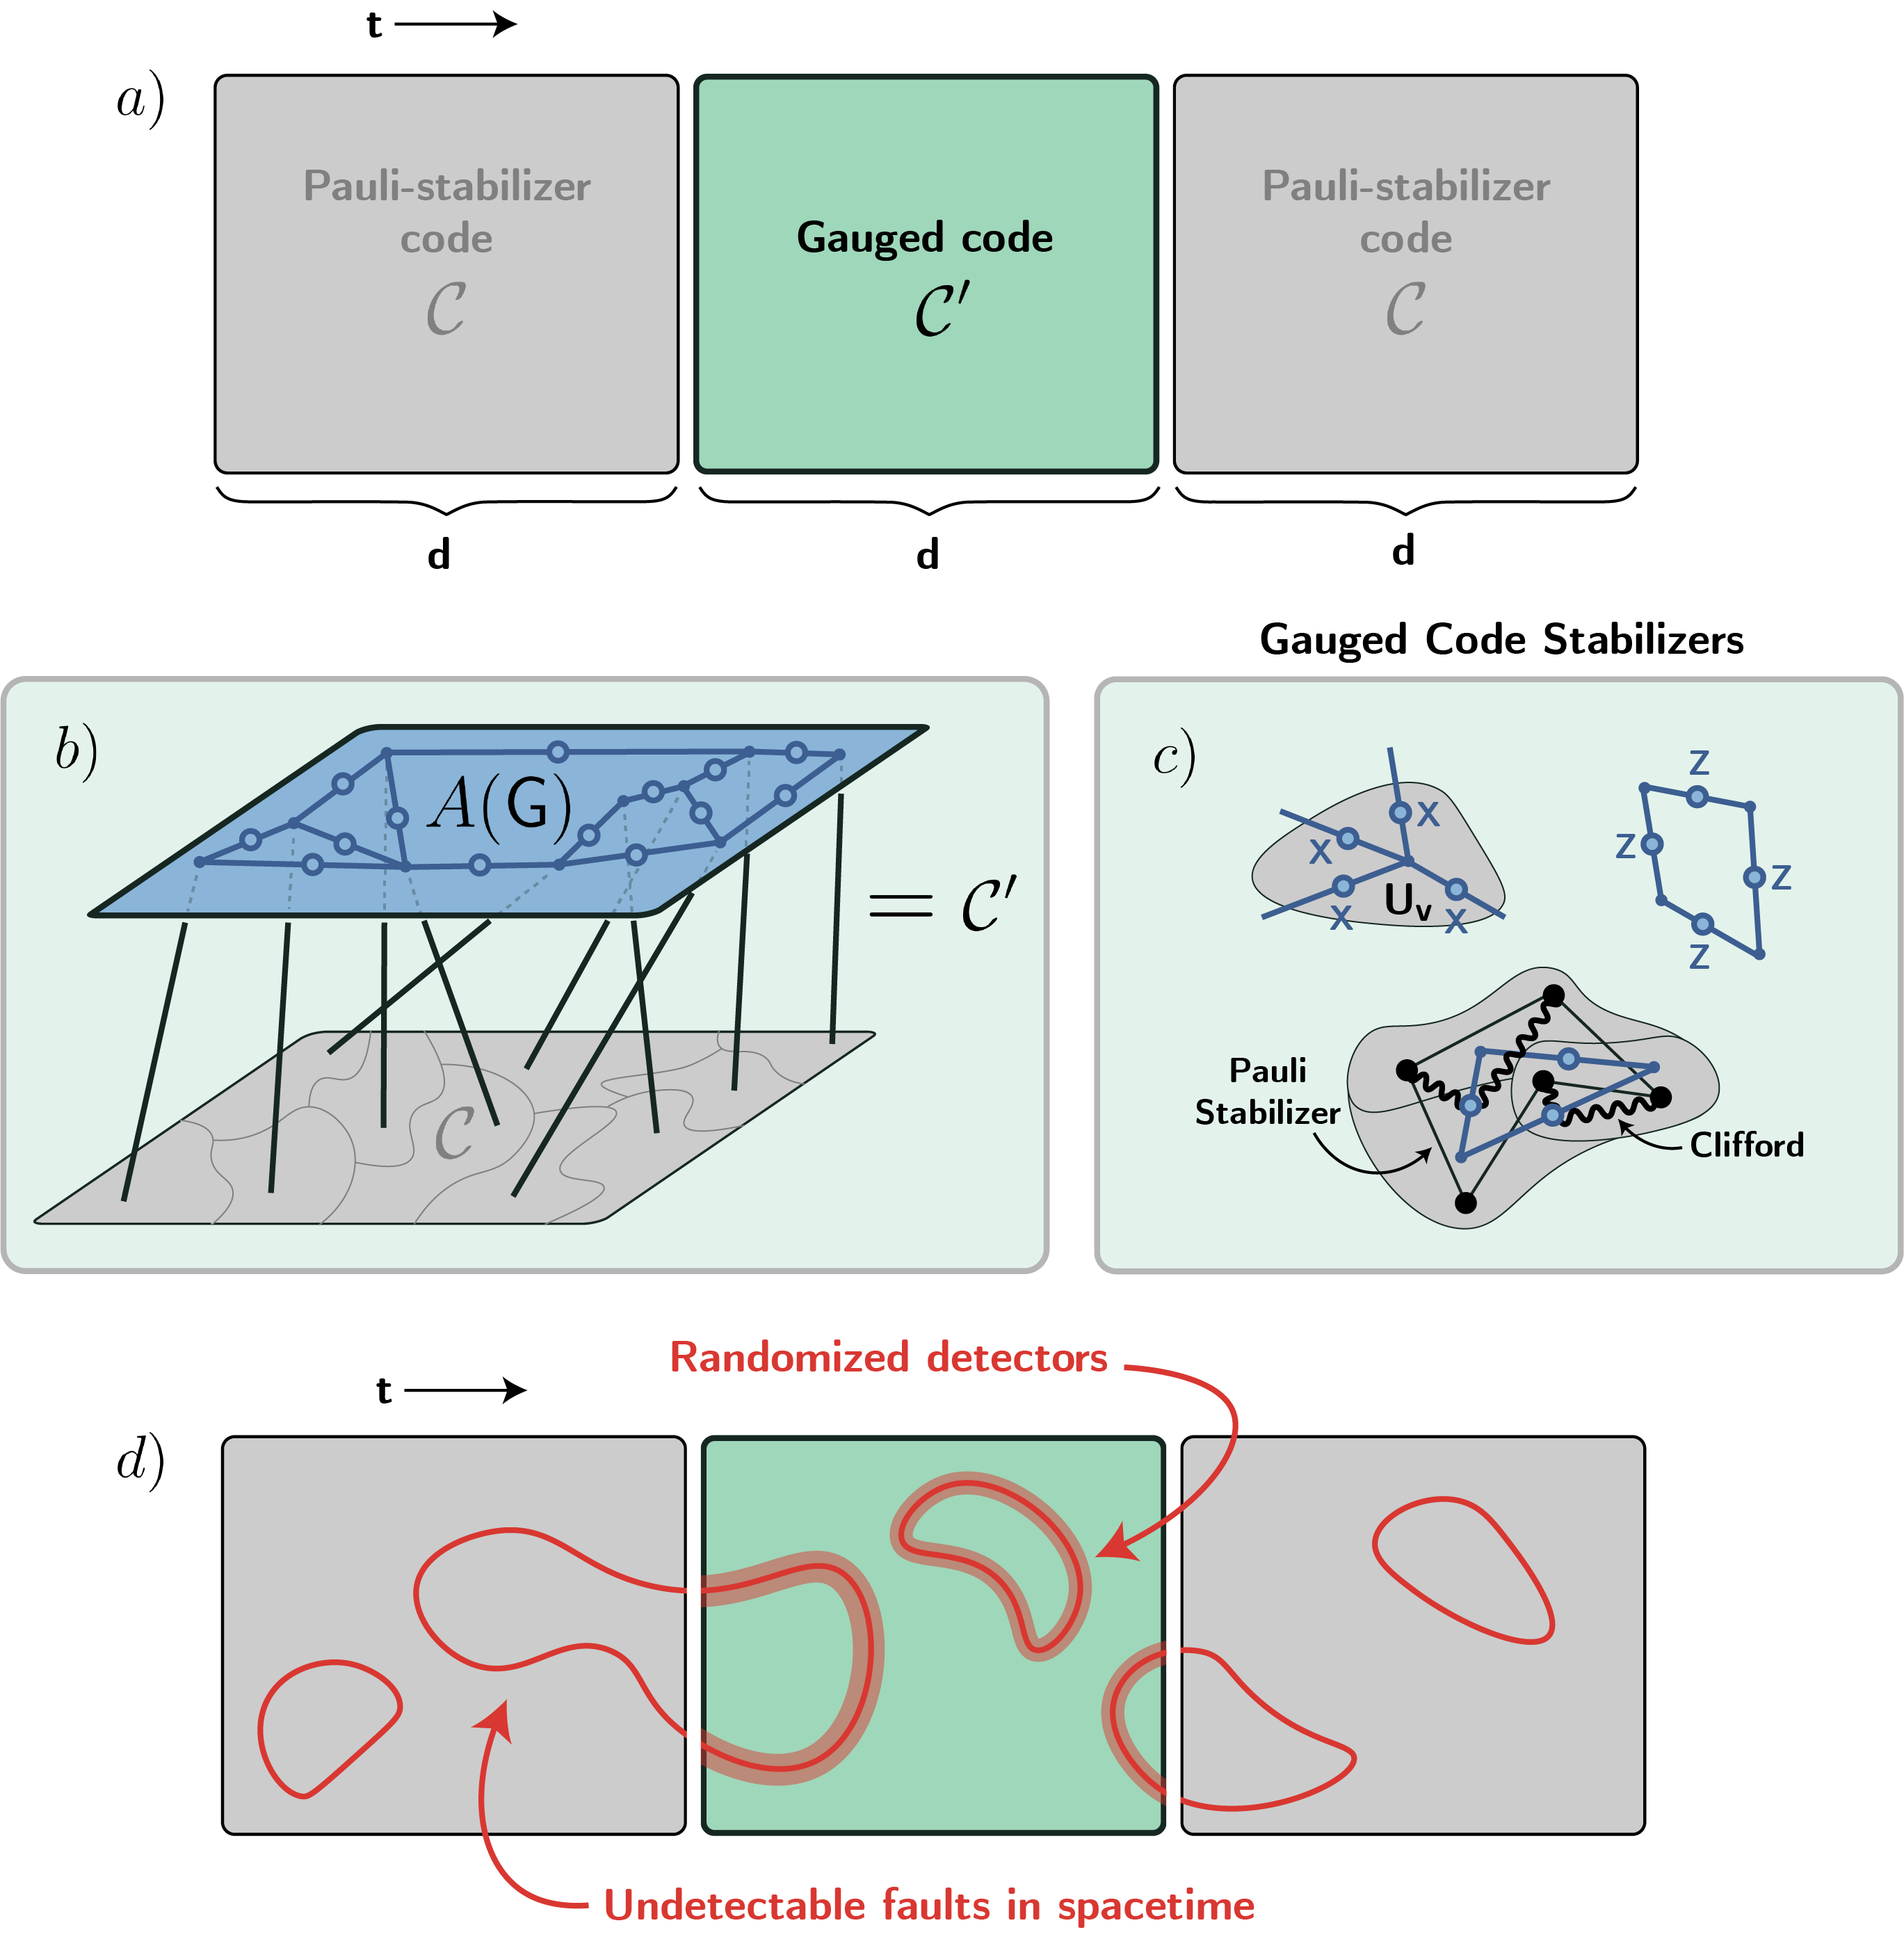
\includegraphics[width=0.75\linewidth]{figs/summary-fig-new.png}
    \caption{
    (a) An abstract depiction of the spacetime volume for the protocol to measure a Clifford operator. Time flows from left to right. We begin with $d$ rounds of syndrome extraction in a Pauli-stabilized code $\cC$ with distance $d$, where $\cC$ has a transversal Clifford operator $\T$ that we wish to measure. We switch into a gauged code $\cC'$ and measure the stabilizers of the gauged code for $d$ rounds. Then, we ungauge, returning to the original code, now projected onto an eigenspace of $\T$. We finish the gadget by measuring $d$ rounds of the $\cC$. (b) The gauged code $\cC'$. The gauged code is constructed by taking the base code $\cC$ and attaching a graph $A(\graphG)$ (blue) with an ancilla at every edge.
    The connection between the base code $\cC$ and the ancilla graph is abstractly depicted with thick black lines that couple to a patch (``vertex set'') of the base code. Each vertex set is associated to a vertex of the ancilla graph, where an ancilla will be placed to measure the gauged checks. These ``vertex'' ancilla can also be viewed as degrees of freedom in an intermediate, ``symmetry-enriched'' version of the base stabilizer code: measuring these ancilla out yields the final deformed Clifford model on the base code and edge ancillas (Sec.~\ref{sec:gauging-procedure}). (c) The attachment of the ancilla graph yields new deformed Clifford stabilizers. 
    Top left: A ``vertex'' stabilizer, the product of all such stabilizers gives the Clifford operator $\T$ being measured. Top right: A ``cycle'' check arising from a cycle of the ancilla graph. Bottom: a deformed stabilizer of the base code, which picks up Clifford decoration spanning the original code degrees of freedom and the ancilla system (Section~\ref{sec:gauging-procedure}).
    (d) We prove that the spacetime protocol in (a) for qubit codes and Clifford operators that satisfy $\T^2=\id$ has a fault distance against data qubit and measurement errors of at least a constant times $d$ (Section~\ref{sec:spacetime-distance}). In the gauged code, certain faults may randomize some detectors in addition to deterministically flipping others. The key observation is that spacetime faults which flip no detectors (represented by red loops in spacetime) only cause detectors in a constant radius around their support to return random outcomes (thickened red outline). }
    \label{fig:summary}
\end{figure}
\subsection{Summary of main results}




In this work, we introduce a method to fault-tolerantly prepare logical magic states in QLDPC codes via measuring transversal Clifford gates. 
The particular QLDPC surgery method we develop is a variant of the gauging logical measurement from Ref.~\cite{williamson2024lowoverheadfaulttolerantquantumcomputation}. 
First, we present a general construction to gauge or measure a transversal Clifford gate of order $p$, $\T^p=\id$, where $p\ge 2$.
This gauging is very adaptable in that the input code can be any \textit{modular} qudit QLDPC code with dimension $q$.
Our construction takes an approach that mirrors generalized code surgery; we introduce auxiliary \textit{gauge qudits} in the $\ket{0}$ state and perform local measurements that deform the initial code into a \textit{gauged code} that contains deformed stabilizers of the original input code, and new stabilizers that include $\T$ in the group they generate. As a result, the measurement of the stabilizers in this gauged code also measures $\T$. 
The code after gauging is a gauged code with a non-Abelian stabilizer group, generalizing the nilpotent and solvable quantum double models~\cite{Kitaev_2003,Tantivasadakarn_2024} that appear when a Clifford logical measurement is performed on a 2D topological code via gauging~\cite{davydova2025universal, sajith2025noncliffordgatesstabilizercodes}.
Our method is efficient in that the number of qudits of this gauged code can be made within a multiplicative logarithmic factor of the block-length of the original code.

\begin{theorem}
    \emph{Space overhead of the deformation (informal; see Section~\ref{sec:defining-gauging-graph}).} Take any QLDPC modular $q$-ary qudit code ($q\ge 2$) encoded in $n$ physical qudits with a transversal Clifford gate $\T$ such that $\T^p=\id$ where $p\ge 2$.  The gauged, QLDPC code that includes $\T$ in its stabilizer group constructed via the procedure defined in Section~\ref{sec:gauging-procedure} 
    has $O(n\log(n))$ qudits for a family of such codes with growing $n$.
\end{theorem}

\noindent In addition to this general gauging recipe, our main theoretical contributions are two-fold.


First, we prove that if the distance of the original QLDPC qudit code is $d$, then the distance of the gauged code is at least $d$ up to a constant factor.
This result applies to any QLDPC code on qudits of any dimension $q$, and transversal gates of any order $p$.

\begin{theorem}
    \emph{Space distance preservation (informal version of Thm.~\ref{thm:space-distance}).}
    Let $\cC$ be a QLDPC modular $q$-ary qudit code, with $q\ge 2$ and distance $d$, with a transversal Clifford gate $\T$. 
    Let $\cC'$ be the gauged code obtained from the procedure in Section~\ref{subsec:gauging-protocol}, using a gauging graph that satisfies the criteria in Definition~\ref{def:graph-desiderata}.
    Then, $\cC'$ is QLDPC and its distance is at least a constant fraction of the distance of $\cC$:
    \[
    d_{\mathrm{g}}\geq \frac{d}{\nu}
    \]
    for some constant $\nu\ge 1$ depending only on the local structure of the gauging construction.
\end{theorem}

\noindent
Along with the distance bound, Section~\ref{sec:space-distance} shows that the gauged code is isomorphic to the symmetric $\T = +1$ subspace of the original code.

While the gauging logical measurement applies to general operators and QLDPC codes~\cite{williamson2024lowoverheadfaulttolerantquantumcomputation}, we focus on the fault tolerance of gauging Clifford operators on qubit stabilizer codes for fault-tolerant magic state preparation.
In practice, the measurement of the Clifford operator $\T$ must occur in the presence of measurement errors. 
To achieve fault-tolerance to measurement and data qubit errors, we must repeat rounds of syndrome extraction in the gauged code at least $d$ times, just as in regular code surgery. 
We define the full gauging measurement procedure as follows: measure stabilizers of the original LDPC code for $d$ rounds, then measure the stabilizers of the gauged code for $d$ noisy rounds, and finally, measure stabilizers of the original code for $d$ rounds.   
Crucially, our results establish that gauging measurement can be made fault-tolerant for the measurement of order-two symmetries, $\T^2 = \id$. This condition is easily satisfied by most Clifford symmetries we are interested in gauging for magic state preparation, such as Hadamard, $\CNOT$, and $\SWAP$.
By fault-tolerant, we mean that a logical fault must contain at least $d/\gamma$ such errors, where $\gamma>0$ is a constant independent of the gauged code parameters.
We prove the following result.
\begin{theorem}
    \emph{Spacetime distance of gauging (informal version of Thm~\ref{thm:spacetime-distance}). Let $\cC$ be a QLDPC qubit stabilizer code with parameters $[[n,k,d]]$ and a transversal Clifford gate $\T$ satisfying $\T^2=\id$.
    The fault-tolerant protocol for measuring $\T$ defined in Section~\ref{sec:spacetime-distance} has adversarial spacetime fault distance 
    \[ d_{\mathrm{f}}\ge \frac{d}{\gamma}
    \]
    where $\gamma\ge 1$ is the a factor independent of code parameters defined in Thm~\ref{thm:spacetime-distance}.
    Equivalently, any undetectable logical failure requires at least $d/\gamma$ elementary faults, including Pauli data qubit errors and measurement faults.}
\end{theorem}

\noindent Establishing fault-tolerance of the spacetime gauging procedure is more complicated for a logical Clifford operator than for a logical Pauli operator for several reasons.


First, by construction, the gauged code must contain non-Pauli stabilizer generators.
As a result, Pauli errors on data qubits neither commute nor anticommute with some neighboring stabilizers.
Therefore, the measurement of these stabilizers is inherently non-deterministic.
Furthermore, the stabilizer generators in the gauged code are only guaranteed to commute within the code space. 
This means that as data qubit errors accumulate in spacetime, detectors of the spacetime volume become non-deterministic and are unusable for detecting errors. 
In this setting, we show that the errors in the spacetime volume of the gauged code can be cleaned in a well-behaved manner due to the structure of the QLDPC Clifford stabilizer group. Specifically, the gauged code is \emph{nilpotent}: all non-Abelian syndromes fuse to the vacuum or to an Abelian syndrome. 
We leave fault-tolerance of gauging $\mathbb{Z}_p$ where $p>2$ Clifford operators in the presence of measurement errors to future work.

In Section~\ref{sec:examples} we construct concrete examples of the gauging procedure.
We gauge a transversal symmetry $W^{\otimes n}$, where $W=XS$, on a \textit{self-dual bivariate bicycle} code constructed by concatenating a bivariate bicycle code with a $[[4,2,2]]$ code as the inner code; we gauge the transversal $\CNOT$ between two bivariate bicycle codes; and we gauge the transversal $XS$ and $HS$ gates on the color code, along with charge conjugation on the qutrit version of the $[[144,12,12]]$ code.
As an example of gauging two symmetries that do not act on all qubits of the code, we gauge a transversal $\CZ$ between two stacks of $3D$ surface codes; finally, we present an algorithm for constructing the gauging graph and the gauged stabilizer group for a fold-transversal $\mathbb{Z}_2$ symmetry on a $2$-dimensional hypergraph product (HGP) code.

An important aspect of this work is constructing concrete examples where measuring Clifford operators on high-rate codes is computationally useful. This is highly nontrivial, due to the difficulty in addressing logical qubits within a high-rate code block. 
In Section~\ref{sec:applicationsA} we introduce an algorithm that gauges the transversal $\CNOT$ between two identical, CSS stabilizer codeblocks to obtain a product state of $k$ copies of the $+1$ eigenstate of $\CNOT$, $\ket{+\CX}^{\otimes k}$.
These eigenstates can subsequently be converted into $O(k)$ copies of Toffoli states, which are the resource state for performing Toffoli gates.
This method is interesting in that it allows the generation of high-fidelity magic states in any CSS LDPC code without distillation or criteria of the LDPC code, such as having a triple intersection point or local multiplication property~\cite{Zhu_2025}.
In Section~\ref{sec:ctrl-t-gadget} we introduce a gadget that uses a sequence of measurements, including a single Clifford measurement, such that we obtain the unitary gate controlled-$U$ where $U$ is a transversal Clifford gate of some QLDPC code with $U^2=\pm 1 $. This gadget is particularly useful, for instance, if we choose $U=\SWAP$, which is readily available between any two identical code blocks, as this enables us to implement a $\SWAP$ network on $N$ registers from requiring $O(N)$ $T$ states to $O(\log_2(N))$ Clifford measurements. 
Using the same gadget, we can also reduce the logical circuit depth of an algorithm that solves the \textit{hidden cut problem}~\cite{bouland2024statehiddensubgroupproblem} by a factor of $\mathcal{O}(n/\epsilon^2)$, where $n$ is the number of qubits of state $\ket{\psi}$, which is $\epsilon$-far from a product state across an unknown bipartition. 
The aim of the hidden cut problem is to find this bipartition given some number of copies of $\ket{\psi}$.
These applications of $\CSWAP$ are an exciting starting point for exploring various structured circuits that are easily compiled into Clifford measurements.
Our results lay down an alternative road to practical and efficient universal FTQC with QLDPC codes. 
For example, our logical magic state preparation protocol via gauging $\CNOT$ can be directly integrated into the \textit{Extractor} architecture~\cite{he2025extractorsqldpcarchitecturesefficient} to produce a fixed-connectivity QLDPC architecture for universal FTQC completely comprised of augmented QLDPC code blocks. 



\subsection{Comparison to existing methods for magic state preparation}

Our results lay down an alternative route to scalable logical magic state preparation in QLDPC codes that offers several advantageous features. First, our scheme is flexible as it only requires the existence of a transversal Clifford gate and hence is applicable to any CSS code. 
Our procedure can also be applied in parallel to Clifford gates with sparse and locally commuting overlap to perform more than one Clifford measurement at a time. 
Second, our scheme is scalable with the size of the code family to which it is applied. The spacetime protocol thus generated relies exclusively on sparse checks and detectors. The fault-distance of our procedure grows linearly with the distance of the target code family. In principle, the distance can be grown a single step at a time. 
The growing distance, combined with the sparse checks, means that our scheme is expected to exhibit a quantum error correcting threshold. That is, a physical error rate below which the logical error rate is suppressed exponentially as a linear function of the distance. Third, our scheme maintains a low overhead as it requires $O(n \log n)$ ancilla qubits~\cite{williamson2024lowoverheadfaulttolerantquantumcomputation,williamson2026fast, yuan2026parsimonious}.


Importantly, in contrast to methods such as magic state cultivation and distillation,  our procedure does not require post-selection. 
This translates directly into a lower qubit footprint for the production of a fixed number of magic states per round when compared to a similar procedure with a lower yield. The above features point to the potential utility of our scheme in the early to mid term fault tolerant era, when physical error rates are relatively close to threshold but the target logical error rate is lower than can be easily achieved through post-selection due to constraints on the number of physical qubits available. 

Magic state distillation is the most prominent approach for the preparation of logical magic states. It relies on the ability to inject noisy physical magic states into a code block upon which logical Pauli stabilizer measurements can be performed. Both the injection and the logical stabilizer measurement stages require post-selection and consequently the yield may be low, although it approaches a constant at the cost of considerable overhead. While the qubit overhead of recently discovered schemes is constant~\cite{wills2024constantoverheadmagicstatedistillation}, for the most widely considered schemes it is polylogarithmic. Distillation also requires multiple logical Pauli measurements, which is expected to incur an additional overhead of $O(n \log n)$ ancilla qubits for $O(d)$ rounds for a generic QLDPC code. There is a further overhead required for logical measurements that cannot be made simultaneously due to high overlap. In comparison to magic state distillation, our scheme provides an alternative path to logical magic states that provides higher yields, a potentially lower qubit footprint, and more fine-grained control over instance sizes. 

Magic state cultivation~\cite{Chamberland_2019,chamberland2020very,gidney2024magic,vaknin2026efficientmagicstatecultivation} is a widely considered approach to preparing logical magic states in the early fault tolerant era.
Cultivation is based on measuring logical Clifford operators to prepare magic states, and relies on post-selection to provide fault tolerance. Consequently, the yield of cultivation exponentially approaches zero making it insufficient for a stand alone scalable solution. In addition, while cultivation can still use a fault-tolerantly prepared cat state to perform measurements on codes with higher distances, it is unclear if the post-selection rates will make this a scalable strategy. In comparison to cultivation, our gauging Clifford measurement scheme has a constant yield that can approach 1 exponentially fast in some cases. Our scheme is scalable and achieves a growing distance while maintaining QLDPC checks and is expected to achieve exponential suppression of the logical error rate as a linear function of the distance for physical error rates below a threshold value~\cite{delafuente2026highthresholddecodingnonpaulicodes}. 

Transversal non-Clifford gates are another approach to preparing logical magic states, or performing non-Clifford operations. They have the advantage of being fault-tolerant with a constant time overhead, no qubit overhead, and yield 1. 
This comes at the cost of requiring complicated code structure that has proven hard to achieve simultaneously with good code properties~\cite{Zhu_2025, Breuckmann_2026, jacob2026singleshotdecodingfaulttolerantgates,Menon_2026,bauer2026findingdiagonallogicalgates,sahay2026computingqldpccodesclimbing}. 
In particular, to take advantage of the constant time overhead of a transversal non-Clifford gate for magic state preparation requires the ability to do single-shot state preparation. Transversal gates on high-rate QLDPC codes also suffer from a targetability problem on the logical qubits. 
In contrast to transversal gates, our approach does not require special code structure for CSS codes, as we can always find a transversal Clifford operator to measure on a CSS stabilizer code. We achieve many of the attractive features of transversal gates, including yield 1, and a low qubit overhead. 

The gauging Clifford measurement was previously considered for 2D topological codes, as part of a general family of fault-tolerant non-Clifford operations~\cite{Bauer_2026}. The advantage of restricting to 2D topological codes is the relative ease of implementation and the addressability of logical qubits~\cite{Fowler_2012}. This comes at the cost of low rates and relative distances due to the constraint of local checks. In comparison to the topological protocols, our work applies to more general QLDPC codes and can be integrated directly into a QLDPC architecture without requiring additional topological code blocks. 
Gauging in high-rate codes means that one can leverage the efficient memory of the QLDPC codes while preparing magic states.

For example, the gauged QLDPC code can be used to simultaneously store computational qubits during the Clifford gauging measurement (Section~\ref{sec:applications}). In particular, even if one $\ket{+\CX}$ magic state is being generated per Clifford measurement, the extra space-overhead used to encode more logical qubits may be utilized in logical compilation. 
Furthermore, we can consider a QLDPC code architecture, in which our magic state factory consists of gauging $\CZ$ on copies of the surface code as in~\cite{brown2020fault,delafuente2026highthresholddecodingnonpaulicodes}. 
Suppose, for example, that a logical compilation requires $K$ magic states of distance $d$ per logical cycle ($d$ syndrome extraction rounds), which would require $O(K)$ surface codes each of size $d\times d$.
Then, in comparison, using the $\CNOT$ gauging scheme on good QLDPC codes~\cite{panteleev2022asymptotically,leverrier2022quantum,dinur2022goodquantumldpccodes} to produce $K$ $\ket{+\CX}$ states per logical cycle has a space overhead of $O(K\times d\log(d))$, which is a multiplicative factor of $d/\log d$ more efficient in spacetime overhead. 




\subsection{Related work}




At the heart of this work is an in-depth development of the gauging logical measurement introduced in Ref.~\cite{williamson2024lowoverheadfaulttolerantquantumcomputation} for Clifford operators on stabilizer codes. This follows earlier work on implementing gauging via an adaptive quantum circuit~\cite{Williamson_2021,Tantivasadakarn_2024,Tantivasadakarn_2023}. The procedure introduced in Ref.~\cite{williamson2024lowoverheadfaulttolerantquantumcomputation} already applied to general non-Pauli operators and codes. However, fault-tolerance was only shown for the measurement of Pauli logical operators on stabilizer codes. The simultaneous work in Ref.~\cite{Ide_2025} found a similar result restricted to CSS codes. 
The proof of spacetime fault tolerance and the construction of explicit applications for Clifford measurements on QLDPC codes set this work apart from the existing literature. 


Prior to this work, Ref.~\cite{davydova2025universal} introduced a fault-tolerant procedure for measuring Clifford operators on topological stabilizer codes in two dimensions via gauging. The fault-tolerance of this procedure relied heavily on the topological properties of two-dimensional topological codes and the anyonic syndromes they support. The results shown here were not derived via a simple extension of the techniques in Ref.~\cite{davydova2025universal}. On the other hand, our constructions and examples provide QLDPC analogs of non-Abelian anyon models such as solvable twisted quantum double models. 
A series of follow-up works developed an array of generalized logic gates based on non-Abelian anyons without proving fault-tolerance~\cite{huang2025generatinglogicalmagicstates,sajith2025noncliffordgatesstabilizercodes}. Further follow-up works have performed numerical simulations of decoding non-Abelian anyons~\cite{delafuente2026highthresholddecodingnonpaulicodes,jing-intrinsic-heralding, jing2026integerlinearprogrammingdecoder}. Extending these ideas to design fault-tolerant gates for QLDPC codes is an interesting future direction. 

Independent of this work, Ref.~\cite{zhu2026nonabelianQLDPCtqftformalism} introduced a procedure to measure Clifford operators via gauging on a large class of QLDPC codes derived from a generalization of the code-to-manifold construction introduced by Freedman and Hastings~\cite{freedman2021buildingmanifoldsquantumcodes}. These codes retain a topological structure that allows arguments similar to those used for two dimensional topological codes to be applied. Ref.~\cite{zhu2026nonabelianQLDPCtqftformalism} argued for a static code distance, but did not establish spacetime fault-tolerance of the logical measurement procedure. They also considered Clifford gates derived from higher-form topological symmetries, and used this to find representative Clifford operators that could be gauged in parallel. Here we have focused on 0-form Clifford gates, however our gauging measurement can as well be applied to any representative of a higher-form Clifford gate and to hypergraphs with no local elements in their kernel. 

In a separate concurrent work, Ref.~\cite{williamson2026fast} introduced a notion of higher-form transversal gates for QLDPC codes together with a fast and fault-tolerant logical measurement procedure via gauging such gates. This procedure is distinct from ours in that it focuses on higher-form transversal gates that provide sufficient meta checks to ensure the gauging procedure is fault tolerant when performed for a single time step. It is a much stricter requirement for a QLDPC code to support a higher-form Clifford gate as compared to a standard 0-form Clifford gate, and so our results here are more generic and apply to all CSS codes. This leads to structurally different fault-tolerance properties, as the deformed checks of the intermediate non-Pauli code do not need to be measured in that case. It is an interesting future direction to combine our techniques with those of Ref.~\cite{williamson2026fast} to develop fault-tolerant higher-form gauging measurements that require more than a constant number of rounds of syndrome extraction in the deformed code, generalizing the partial block reading results derived for Pauli codes in Ref.~\cite{cowtan2025fast}. 

In another concurrent work, Ref.~\cite{christos2026nonabelianquantumlowdensityparity} considered non-Pauli QLDPC codes that arise from gauging Clifford logical operators. They present two distinct gauging methods: a homological method and a graph cluster-state based method. We use the same graph based method, previously introduced in Refs.~\cite{Williamson_2021,Tantivasadakarn_2024,verresen2022efficientlypreparingschrodingerscat,Tantivasadakarn_2023} in a topological setting. Reference~\cite{christos2026nonabelianquantumlowdensityparity} do not prove fault-tolerance of the graph gauging method and neither do they provide specific details of the Clifford measurement protocol implemented via gauging or give particular practical applications of this method. As discussed above, the original gauging measurement procedure in Ref.~\cite{williamson2024lowoverheadfaulttolerantquantumcomputation} was already applicable to non-Pauli gates and codes. Deriving the form of the deformed codes when a non-Pauli gate is gauged follows from a standard recipe which we have used here, see for example the explanation in Ref.~\cite{Bulmash_2019,Prem_2019,verresen2022efficientlypreparingschrodingerscat}. 


\subsection{Organization of the paper}

The remainder of this paper is organized as follows.
Section~\ref{sec:gauging-procedure} presents the procedure for measuring logical Cliffords, and derives the stabilizers of the intermediate gauged code.

Section~\ref{sec:space-distance} establishes the properties of the gauged code, namely its isomorphism with the symmetric $\T= +1$ subspace of the original code, and the fact that code distance is preserved under our gauging protocol.
Section~\ref{sec:spacetime-distance} addresses fault tolerance of the gauging procedure, proving a lower bound on the spacetime fault distance of the gauging measurement of a $\mathbb{Z}_2$ symmetry $\T$ of a qubit CSS code.
Section~\ref{sec:examples} presents examples of gauging on bivariate bicycle codes, the color code, and hypergraph product codes.
Section~\ref{sec:applications} presents applications: (1) a scheme to prepare multiple $\tof$ states on a single CSS QLDPC codeblock using our fault-tolerant gauging protocol, and (2) a gadget that uses a single Clifford measurement of transversal $\SWAP$ to perform many $\CSWAP$ operations in parallel.
We conclude with a discussion, and some more detailed derivations are collected in Appendix~\ref{app:gauging-procedure-proofs}.

\subsubsection*{Reader's Guide }

Section \ref{sec:gauging-procedure} is a pre-requisite for all following sections. However, a reader not interested in following the proof of the fault distance for the protocol can skip directly from Section \ref{sec:gauging-procedure} to Section~\ref{sec:examples} to understand the examples of the construction, or Section~\ref{sec:applications} to see applications of Clifford measurement in magic state preparation and algorithmic subroutines.
Sections \ref{sec:space-distance} and Section \ref{sec:spacetime-distance} may be read independently.

\subsection*{Acknowledgments}

Part of this work was performed while AL and KC were summer interns at IBM Quantum.
KC and AL thank Mackenzie Shaw, Louis Golowich, Adam Wills, Zhiyang He, Christopher Pattison and Alfred for encouraging discussions and support. 
KC and BJB thank Sergey Bravyi for bringing to our attention an application of our gadgets to the hidden cut problem.
KC thanks Shifan Xu for enlightening discussions on the SWAP network circuit.
Part of this work was done during the ``Noise-robust Phases of Quantum Matter'' program at the Kavli Institute for Theoretical Physics (KITP).
BJB is grateful for the hospitality of the Niels Bohr Institute at the University of Copenhagen.
DJW is supported by the Australian Research Council Discovery Early Career Research Award (DE220100625). 
AL acknowledges the NSF GRFP (Grant No. DGE 2140743) and the Kavli Institute for Theoretical Physics Graduate Fellowship Program, supported in part by Grant No. NSF PHY-1748958 to the Kavli Institute for Theoretical Physics (KITP), the Heising-Simons Foundation, and the Simons Foundation (216179, LB).
YR was supported by the U.S.
Department of Energy, Office of Science, National Quantum Information Science Research Centers, Quantum Systems Accelerator, under Grant
number DOE DE-SC0012704.
HP was supported by the Department of Defense through the National Defense Science and Engineering Graduate (NDSEG) Fellowship Program.

\subsection*{AI statement}


The scientific content of this work was conceived by the authors without the use of generative AI. 
Generative AI tools (ChatGPT 5.6, GPT-6 Sol, GPT-6 Astra, Claude Fable 5) were used during the final stages of the manuscript preparation to verify proofs, and for language and presentation edits. AI assistance for basic spellchecking and grammar was provided by Grammarly. 
All
content, claims, and conclusions have been reviewed and
verified by the authors to ensure accuracy and originality. 
Certain products, commercial and otherwise, are
mentioned in this publication. These mentions are for
informational purposes only, and do not imply recommendation or endorsement by NIST.



\ifdefined\ismainfile
\else
    \end{document}
\fi
